\documentclass[10pt, twocolumn]{article}

% --- Packages ---
\usepackage[margin=0.75in]{geometry}
\usepackage{graphicx}
\usepackage{booktabs}
\usepackage{hyperref}
\usepackage{amsmath}
\usepackage{xcolor}
\usepackage{caption}
\usepackage{float}
\usepackage{enumitem}
\usepackage{url}
\usepackage{times}

\hypersetup{
    colorlinks=true,
    linkcolor=black,
    citecolor=black,
    urlcolor=blue
}

% Compact spacing
\setlength{\parskip}{4pt}
\setlength{\parindent}{0pt}
\setlist{nosep, leftmargin=*}

% --- Title ---
\title{\Large\textbf{Reading the Game: Real-Time Win Prediction\\from Broadcast Video}}
\author{
    Trevor Gregory \\
    College of Business and Computing \\
    Regis University, Denver, CO \\
    \texttt{tgregory004@regis.edu}
}
\date{}

\begin{document}
\maketitle

% ============================================================
% ABSTRACT
% ============================================================
\begin{abstract}
Professional esports broadcasts offer rich visual information---scores, timers, player positions on a minimap---but no structured data feed for real-time analytics. This paper presents an end-to-end computer vision pipeline that processes raw Call of Duty League broadcast footage at 1080p/60fps and produces frame-level win probability estimates. The system combines YOLOv8 object detection for minimap player tracking with template matching OCR for scoreboard extraction, feeding 12 engineered features into an XGBoost classifier. Validated on a held-out match across 111,360 total frames, I found that minimap telemetry features contribute approximately 43\% of the model's predictive power---a finding that suggests spatial awareness data captures match dynamics that the scoreboard alone cannot. The complete pipeline renders a broadcast-quality win probability overlay at 59.94 fps.
\end{abstract}

% ============================================================
% I. INTRODUCTION
% ============================================================
\section{Introduction}

Anyone who has watched an NFL broadcast in the last few years has seen it: a small graphic in the corner showing each team's real-time probability of winning. ESPN, CBS, and the major networks have had this capability for years, powered by access to proprietary play-by-play data feeds. Esports, despite being a rapidly growing competitive industry, has nothing equivalent. The Call of Duty League (CDL) broadcasts its matches on YouTube, but unlike traditional sports, there is no public API and no structured data feed available to third-party analysts.

This creates an interesting challenge. The broadcast video itself contains everything a viewer needs to understand the match state---team scores displayed on the HUD, a game clock counting down, and a minimap in the corner showing player positions. The data is all there, rendered as pixels on screen. The question is whether computer vision can extract it reliably enough to power a real-time predictive model.

That is the goal of this project: a complete pipeline that takes raw broadcast footage as its only input and produces a live win probability overlay as its output. No game API, no replay files, no manual annotation of match events. Just pixels in, predictions out.

The core contribution is the discovery that minimap telemetry---player counts extracted via object detection---adds substantial predictive value beyond what the scoreboard provides. Specifically, I found that minimap-derived features account for approximately 43\% of the model's overall feature importance, demonstrating that spatial awareness data captures team fight dynamics that precede and predict scoring runs.

% ============================================================
% II. RELATED WORK
% ============================================================
\section{Related Work}

Real-time win probability has a long history in traditional sports analytics, where structured event data (pitch-by-pitch in baseball, play-by-play in football) feeds directly into probabilistic models. In esports, the landscape is less mature. Most existing work in esports analytics relies on game-specific APIs or replay file parsers---tools that provide clean structured data but are not universally available across all titles and tournaments.

Computer vision approaches to esports analysis remain relatively unexplored. Object detection frameworks such as YOLO \cite{jocher2023yolo} have been widely adopted for real-time detection tasks, and their speed makes them a natural fit for processing game footage. For annotation at scale, active learning strategies \cite{settles2009active} offer a practical path to reducing the manual labeling burden. On the modeling side, gradient-boosted tree ensembles like XGBoost \cite{chen2016xgboost} are well-suited for structured tabular features, which is exactly the type of data this pipeline produces.

The approach described here differs from prior work by operating entirely on broadcast video with no access to game internals, combining neural (YOLOv8) and symbolic (template matching) extraction methods into a single pipeline, and demonstrating that spatial minimap features meaningfully improve prediction accuracy over scoreboard data alone.

% ============================================================
% III. METHODOLOGY
% ============================================================
\section{Methodology}

The pipeline consists of five stages: data acquisition, minimap detection, scoreboard extraction, feature engineering, and win probability modeling. Figure~\ref{fig:pipeline} shows the full architecture.

\begin{figure}[H]
    \centering
    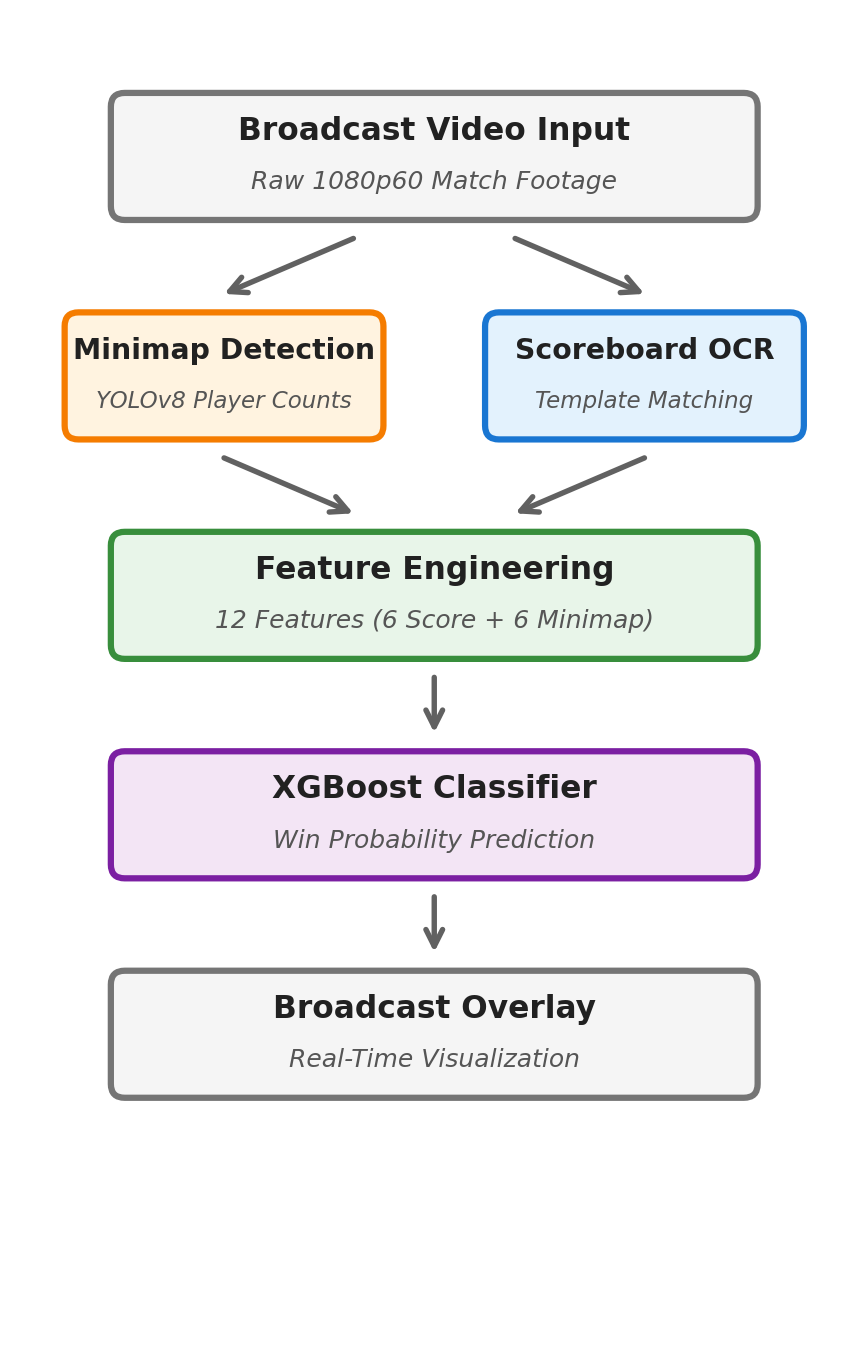
\includegraphics[width=\columnwidth]{figures/Pipeline_diagram.png}
    \caption{End-to-end pipeline architecture. Raw broadcast footage is processed through two parallel extraction paths---YOLOv8 for minimap player detection and template matching for scoreboard OCR---before being combined into a structured telemetry dataset that feeds the XGBoost probability classifier.}
    \label{fig:pipeline}
\end{figure}

\subsection{Data Acquisition}

Match footage was sourced from official CDL broadcasts on YouTube using \texttt{yt-dlp}, extracting full-resolution 1080p video at 59.94 fps. Three complete Hardpoint matches were selected from two different broadcast sessions, totaling 111,360 frames of game time. Hardpoint is a rotating objective mode where teams earn points by occupying a designated area, and the first team to 250 points wins.

\subsection{Minimap Player Detection}

The broadcast HUD includes a minimap in the lower-left corner that shows real-time player positions: white arrows for the observed team and red diamonds for opponents. I trained a YOLOv8 model to detect and count these icons, providing per-frame player and enemy counts.

\textbf{Active Learning Annotation.} Manually labeling 700+ minimap crops is tedious. Instead, I adopted a human-in-the-loop approach inspired by active learning \cite{settles2009active}: I manually labeled a seed set of 50 frames in LabelMe, trained a lightweight YOLOv8-Nano model on this seed set, ran inference on the remaining 688 unlabeled images, and then corrected the model's predictions rather than drawing boxes from scratch. This reduced annotation time by roughly 90\%.

The production model was a YOLOv8-Medium trained on the full corrected dataset using PyTorch \cite{paszke2019pytorch} with Apple Silicon MPS acceleration. Two classes were defined: \texttt{player} (friendly) and \texttt{enemy}.

\subsection{Scoreboard OCR}

The broadcast HUD displays both team scores and a game clock at fixed screen coordinates. Extracting these values accurately at 60 fps turned out to be the most iterative part of the project.

\textbf{EasyOCR Attempt.} My initial approach used EasyOCR for text recognition on cropped score regions. While this worked on some frames, the game's stylized numeric font produced frequent misreads---digits like ``8'' and ``6'' were routinely confused, and multi-digit scores (e.g., ``142'') were often parsed incorrectly. The resulting telemetry was too noisy for reliable modeling.

\textbf{Template Matching.} I pivoted to a template matching approach using OpenCV's \cite{bradski2000} normalized cross-correlation (NCC). For each digit 0--9, I extracted multiple reference templates at native resolution from known-good frames. The matching process works as follows:

\begin{enumerate}
    \item Crop the fixed-coordinate score and timer ROIs from each frame.
    \item Binarize using adaptive thresholding for clean digit isolation.
    \item Count the number of digit slots by measuring content-width columns.
    \item For each slot, slide all candidate templates and select the best match via geometric mean confidence with a coverage constraint.
    \item Post-process the full sequence with monotonicity enforcement and outlier spike removal.
\end{enumerate}

This approach achieved 99.3\% field completeness across all 111,360 frames, with the remaining gaps filled via forward-fill interpolation.

\subsection{Feature Engineering}

Each frame produces a raw observation: two team scores, a game clock, and two player counts from the minimap. From these, I engineered 12 features organized into two groups (Table~\ref{tab:features}).

\begin{table}[h]
\centering
\caption{Engineered feature set (12 features).}
\label{tab:features}
\small
\begin{tabular}{@{}lll@{}}
\toprule
\textbf{\#} & \textbf{Feature} & \textbf{Source} \\
\midrule
1 & \texttt{score\_a} & Scoreboard \\
2 & \texttt{score\_b} & Scoreboard \\
3 & \texttt{score\_diff} & Scoreboard \\
4 & \texttt{score\_rate\_a} & Scoreboard \\
5 & \texttt{score\_rate\_b} & Scoreboard \\
6 & \texttt{time\_remaining\_fraction} & Scoreboard \\
\midrule
7 & \texttt{player\_count\_map} & Minimap \\
8 & \texttt{enemy\_count\_map} & Minimap \\
9 & \texttt{player\_advantage} & Minimap \\
10 & \texttt{player\_alive\_rolling} & Minimap \\
11 & \texttt{enemy\_alive\_rolling} & Minimap \\
12 & \texttt{advantage\_rolling} & Minimap \\
\bottomrule
\end{tabular}
\end{table}

The rolling features use a 30-second window (approximately 1,800 frames at 59.94 fps) to smooth the inherent noise in per-frame minimap counts. Players respawn every few seconds in Hardpoint, so raw counts fluctuate rapidly. The rolling average captures sustained map control---a team consistently maintaining more players on the map is likely controlling objective time, which drives scoring.

\subsection{Win Probability Model}

I trained an XGBoost \cite{chen2016xgboost} binary classifier to predict, at each frame, the probability that Team A wins the match. The model uses 300 trees with a maximum depth of 4 and a learning rate of 0.05.

\textbf{Mirror Augmentation.} With only three matches, class balance and data volume are concerns. To address this, I created a mirrored copy of each training match by swapping Team A and Team B perspectives---scores, rates, and minimap counts are all flipped, and the win label is inverted. This doubles the training set from 77,040 to 154,080 rows and ensures both win/loss outcomes are represented regardless of which team actually won each match.

\textbf{Hold-Out Validation.} I trained on Matches 1 and 3 (different winners, different broadcast sessions) and held out Match 2 as a pure test set. This is a stricter validation than a random frame-level split, since the model must generalize to a completely unseen match with a different outcome trajectory.

% ============================================================
% IV. RESULTS
% ============================================================
\section{Results}

\subsection{Feature Importance}

The trained model reveals an interesting split in feature importance (Table~\ref{tab:importance}). While \texttt{score\_diff} is the single most important feature at 0.26, the three rolling minimap features collectively contribute 0.44---nearly half of the model's total predictive signal. This means that even with access to the exact score, the model gains substantial additional information from knowing how many players each team has on the map over the last 30 seconds.

\begin{table}[h]
\centering
\caption{Top feature importances (XGBoost gain).}
\label{tab:importance}
\small
\begin{tabular}{@{}llr@{}}
\toprule
\textbf{Feature} & \textbf{Source} & \textbf{Importance} \\
\midrule
\texttt{score\_diff} & Scoreboard & 0.26 \\
\texttt{player\_alive\_rolling} & Minimap & 0.16 \\
\texttt{enemy\_alive\_rolling} & Minimap & 0.15 \\
\texttt{advantage\_rolling} & Minimap & 0.13 \\
\texttt{score\_rate\_a} & Scoreboard & 0.07 \\
\texttt{score\_b} & Scoreboard & 0.05 \\
\bottomrule
\end{tabular}
\end{table}

\subsection{Hold-Out Match Validation}

Figure~\ref{fig:validation} shows the model's predictions on the held-out match. The top panel displays the actual scores over time; the bottom panel shows the predicted Team A win probability. Early in the match, when the score is close, the model assigns near-even odds. As Team A builds a scoring lead around the 250-second mark, the probability shifts decisively in their favor and remains there through the match's conclusion. The model correctly identifies the eventual winner for the majority of the match duration.

\begin{figure}[H]
    \centering
    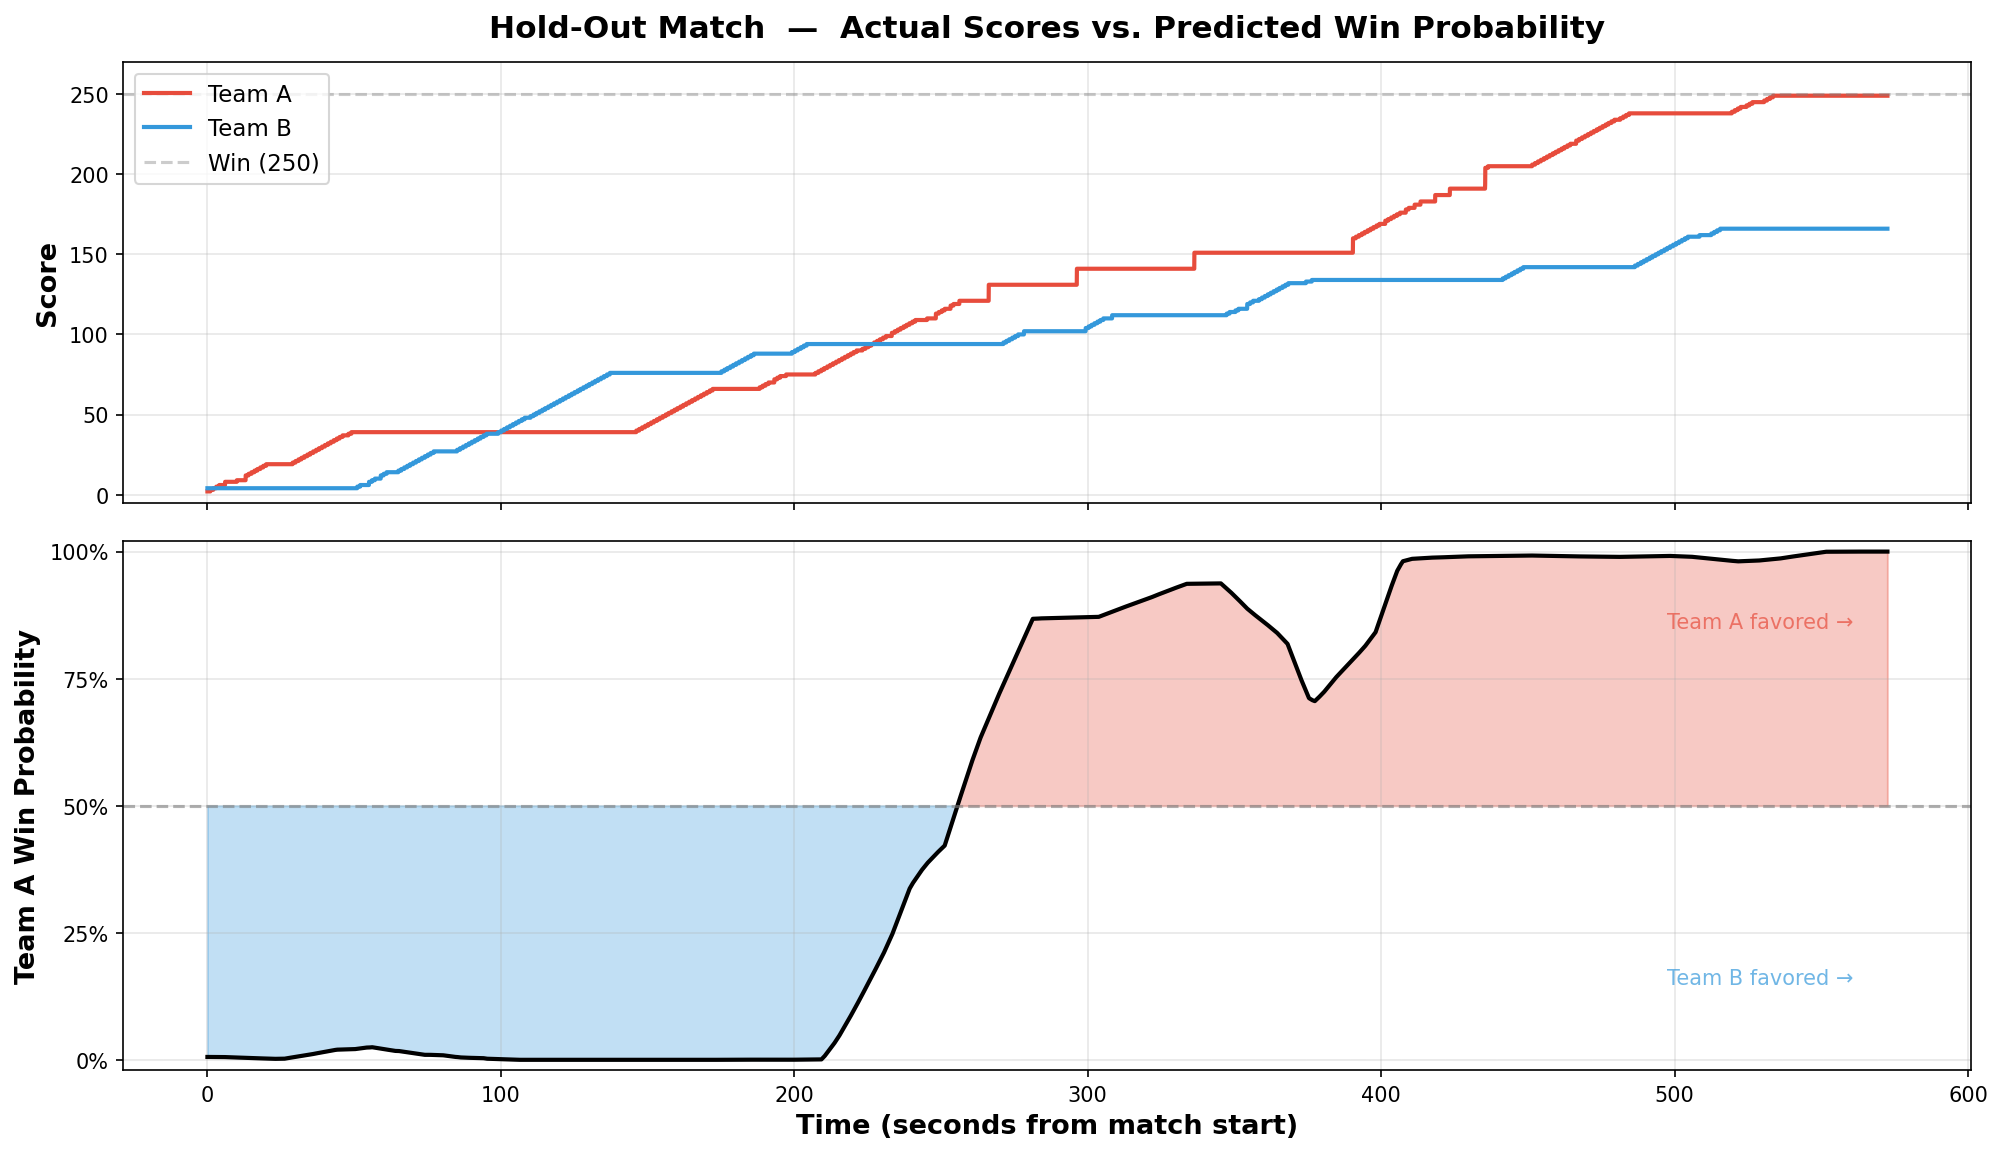
\includegraphics[width=\columnwidth]{figures/final_validation_chart.png}
    \caption{Hold-out match validation. Top: actual scores. Bottom: predicted Team A win probability (smoothed with 30-second rolling average).}
    \label{fig:validation}
\end{figure}

\subsection{Broadcast Overlay}

As a practical demonstration, I rendered the win probability as a broadcast-style overlay directly onto the match footage using OpenCV \cite{bradski2000}. The overlay includes team scores, win percentages, and a color-coded probability bar, rendered at the video's native 59.94 fps. A 30-second demo clip was produced for presentation purposes, with additional exponential smoothing applied to the bar animation for a polished visual result.

% ============================================================
% V. DISCUSSION
% ============================================================
\section{Discussion}

\textbf{The Template Matching Pivot.} One of the more instructive parts of this project was the shift from EasyOCR to template matching. EasyOCR is a well-regarded general-purpose OCR library, and I expected it to handle numeric digit recognition without issue. In practice, the game's stylized font and the small size of the score regions produced too many errors for reliable downstream modeling. The template matching approach, while more manual to set up (extracting reference templates, tuning thresholds), proved far more robust. This is a good reminder that domain-specific solutions often outperform general-purpose tools when the problem is well-constrained.

\textbf{Why Minimap Telemetry Matters.} The finding that minimap features contribute roughly 43\% of predictive power is, I think, the most interesting result. Intuitively, it makes sense: a team that is losing players faster than the opponent will eventually lose map control, which means less time on the objective, which means fewer points. This dynamic plays out over a 10--30 second window---well before the scoreboard reflects it. The rolling average features capture exactly this leading indicator.

\textbf{Limitations.} This work has several clear limitations. Three matches is a small sample, and all three are from a single game mode (Hardpoint). The model has not been tested on other modes such as Search \& Destroy or Control, where the scoring dynamics differ substantially. Additionally, the hold-out validation uses a match from the same video as one of the training matches (different map, same broadcast), which may share visual characteristics. A stronger validation would use matches from entirely different tournaments or seasons.

\textbf{Use of AI Tools.} I used Claude \cite{anthropic2026} and Gemini \cite{google2026} as development assistants throughout this project---for debugging, code generation, and iteration on pipeline design. All architectural decisions, feature engineering choices, and analytical conclusions are my own. The AI tools accelerated implementation but did not replace the domain reasoning required to design the pipeline or interpret its outputs.

% ============================================================
% VI. CONCLUSION
% ============================================================
\section{Conclusion}

This project demonstrates that a complete win probability pipeline can be built from broadcast video alone, without access to any game API or structured data feed. The central finding---that minimap-derived spatial telemetry contributes roughly 43\% of the model's predictive power---suggests that there is meaningful signal in the broadcast beyond what the scoreboard shows, and that computer vision can extract it at scale.

Looking forward, several extensions would strengthen the system: training on a larger corpus of matches across multiple tournaments and game modes, incorporating temporal models (LSTMs or transformers) to capture sequential patterns in feature trajectories, and ultimately deploying the pipeline for live streaming inference. The tools and techniques used here---YOLOv8, template matching, XGBoost---are all production-ready and performant enough for real-time operation.

The broader vision is bringing the kind of real-time predictive analytics that traditional sports have enjoyed for years into the esports space, starting with nothing more than a YouTube stream.

% ============================================================
% REFERENCES
% ============================================================
\bibliographystyle{IEEEtran}
\bibliography{references}

\end{document}
